% Options for packages loaded elsewhere
\PassOptionsToPackage{unicode}{hyperref}
\PassOptionsToPackage{hyphens}{url}
%
\documentclass[
]{article}
\usepackage{amsmath,amssymb}
\usepackage{lmodern}
\usepackage{iftex}
\usepackage{fancyhdr}

\usepackage{titlesec}
\ifPDFTeX
  \usepackage[T1]{fontenc}
  \usepackage[utf8]{inputenc}
  \usepackage{textcomp} % provide euro and other symbols
\else % if luatex or xetex
  \usepackage{unicode-math}
  \defaultfontfeatures{Scale=MatchLowercase}
  \defaultfontfeatures[\rmfamily]{Ligatures=TeX,Scale=1}
\fi
% Use upquote if available, for straight quotes in verbatim environments
\IfFileExists{upquote.sty}{\usepackage{upquote}}{}
\IfFileExists{microtype.sty}{% use microtype if available
  \usepackage[]{microtype}
  \UseMicrotypeSet[protrusion]{basicmath} % disable protrusion for tt fonts
}{}
\makeatletter
\@ifundefined{KOMAClassName}{% if non-KOMA class
  \IfFileExists{parskip.sty}{%
    \usepackage{parskip}
  }{% else
    \setlength{\parindent}{0pt}
    \setlength{\parskip}{6pt plus 2pt minus 1pt}}
}{% if KOMA class
  \KOMAoptions{parskip=half}}
\makeatother
\usepackage{xcolor}
\usepackage{longtable,booktabs,array}
\usepackage{calc} % for calculating minipage widths
% Correct order of tables after \paragraph or \subparagraph
\usepackage{etoolbox}
\makeatletter
\patchcmd\longtable{\par}{\if@noskipsec\mbox{}\fi\par}{}{}
\makeatother
% Allow footnotes in longtable head/foot
\IfFileExists{footnotehyper.sty}{\usepackage{footnotehyper}}{\usepackage{footnote}}
\makesavenoteenv{longtable}
\usepackage{graphicx}
\makeatletter
\def\maxwidth{\ifdim\Gin@nat@width>\linewidth\linewidth\else\Gin@nat@width\fi}
\def\maxheight{\ifdim\Gin@nat@height>\textheight\textheight\else\Gin@nat@height\fi}
\makeatother
% Scale images if necessary, so that they will not overflow the page
% margins by default, and it is still possible to overwrite the defaults
% using explicit options in \includegraphics[width, height, ...]{}
\setkeys{Gin}{width=\maxwidth,height=\maxheight,keepaspectratio}
% Set default figure placement to htbp
\makeatletter
\def\fps@figure{htbp}
\makeatother
\usepackage[normalem]{ulem}
\setlength{\emergencystretch}{3em} % prevent overfull lines
\providecommand{\tightlist}{%
  \setlength{\itemsep}{0pt}\setlength{\parskip}{0pt}}
\setcounter{secnumdepth}{-\maxdimen} % remove section numbering
\ifLuaTeX
  \usepackage{selnolig}  % disable illegal ligatures
\fi
\IfFileExists{bookmark.sty}{\usepackage{bookmark}}{\usepackage{hyperref}}
\IfFileExists{xurl.sty}{\usepackage{xurl}}{} % add URL line breaks if available
\urlstyle{same} % disable monospaced font for URLs
\hypersetup{
  hidelinks,
  pdfcreator={LaTeX via pandoc}}

\author{}
\date{}
\pagestyle{fancy}
\fancyhf{} % Clear default headers and footers
\fancyhead[C]{\textbf{NLP \& Text-Based Modeling}} % Title in header
\renewcommand{\headrulewidth}{0.4pt} % Adds a line under the header
\fancyfoot[C]{\textit{School of Computer Engineering, KIIT, BBSR} \thepage}
\renewcommand{\footrulewidth}{0pt} % No line under the footer



\begin{titlepage}
    \begin{center}
        \textbf{\Large A PROJECT REPORT}\\[1cm]
        \textbf{\Large on}\\[0.5cm]
        \textbf{\Large ``NLP \& Text-Based Modeling''}\\[1.5cm]
        \textbf{Submitted to}\\[0.5cm]
        \textbf{KIIT Deemed to be University}\\[0.5cm]
        \textbf{In Partial Fulfilment of the Requirement for the Award of}\\[0.5cm]
        \textbf{BACHELOR'S DEGREE IN COMPUTER SCIENCE \& ENGINEERING}\\[1cm]
        \textbf{BY}\\[0.5cm]
         

\begin{center}
    \begin{tabular}{|c|c|}
        \hline
        \textbf{Name} & \textbf{Roll Number} \\
        \hline
        Soujanya Datta & 22053284 \\
        Sudeep Patra & 22053293 \\
        \hline
    \end{tabular}\\[2cm]
\end{center}

\begin{figure}
            \centering
            
\includegraphics[width=0.5\linewidth]{kiit_logo.jpg}
            \label{fig:enter-label}
        \end{figure}
                \textbf{SCHOOL OF COMPUTER ENGINEERING}\\
        \textbf{KALINGA INSTITUTE OF INDUSTRIAL TECHNOLOGY}\\
        \textbf{BHUBANESWAR, ODISHA - 751024}\\[0.5cm]
        \textbf{March 2025}
    \end{center}
\end{titlepage}

\newpage
\begin{center}
    \textbf{CERTIFICATE}\\[1cm]

    \begin{figure}
        \centering
        
\includegraphics[width=0.75\linewidth]{kiit_logo.jpg}
        \label{fig:enter-label}
    \end{figure}


    
    This is to certify that the project entitled\\
    \textbf{``NLP \& Text-Based Modeling''}\\
    submitted by\\
    Soujanya datta (22053284) and Sudeep Patra (22053293), \\
    is a record of bonafide work carried out by them, in partial fulfilment of the requirement for the award of\\
    Bachelor of Engineering in Computer Science \& Engineering at KIIT Deemed to be University, Bhubaneswar.\\[1cm]
    This work is done during the year 2024-2025, under our guidance.\\[2cm]
    \textbf{Jyotiprakash Mishra}\\
    \textbf{Project Guide}
\end{center}

\newpage
\begin{center}
    \textbf{ACKNOWLEDGEMENTS}
\end{center}
\noindent
We are profoundly grateful to \textbf{Jyotiprakash Mishra Sir} of \textbf{KIIT School of Computer Engineering} for his expert guidance and continuous encouragement throughout this project.\\[1cm]

\begin{center}
\textbf{SOUJANYA DATTA &, SUDEEP PATRA }
\end{center}


\newpage
\begin{center}
    \textbf{ABSTRACT}
\end{center}
\noindent
ABSTRACT
Natural Language Processing (NLP) is a rapidly evolving field that bridges
human communication and computational intelligence. This project explores
various NLP tasks, from fundamental text preprocessing—such as tokenization,
stopword removal, and vectorization—to advanced model development using
both classical machine learning techniques (Logistic Regression, Naïve Bayes)
and modern transformer-based architectures (BERT, DistilBERT). Additionally,
topic modeling methods like LDA and BERTopic are employed to uncover
hidden themes within textual data. A key focus is on model interpretability,
using techniques like LIME, SHAP, and attention heatmaps to visualize how
models make predictions.
To ensure explainability in NLP models, we employ various techniques to
identify influential words in predictions. Performance is evaluated using
accuracy, F1-score, and confusion matrices for classification, while coherence
scores assess topic models. A strong emphasis is placed on exploratory data
analysis, model comparisons, and visualization to communicate results
effectively. Finally, the project discusses the limitations of existing approaches
and proposes future improvements for text-based modeling.\\[1cm]
\textbf{Keywords:} NLP, Text Classification, Pre-processing, Topic Modeling,
Transformer Models (BERT/DistilBERT), Explainability, LIME, SHAP

\newpage

\tableofcontents
\newpage

\section{1 Introduction}


The project encompasses a complete NLP pipeline, starting from data preprocessing using tokenization, stopword removal, and lemmatization, to feature engineering with TF-IDF and word embeddings. Various classical machine learning models, such as Logistic Regression and Naïve Bayes, are first evaluated on the datasets. Then, modern transformer-based models like DistilBERT and BERT are applied to the same datasets to conduct a comparative study. This analysis helps in understanding the limitations and improvements of different classification techniques, as well as identifying future research directions based on how datasets behave under varying modeling approaches.


Additionally, topic modeling techniques like LDA and BERTopic are used to extract latent topics, providing deeper insights into the underlying text structures. Explainability techniques such as LIME, SHAP, and attention heatmaps are integrated to highlight the most influential words in model predictions, ensuring greater interpretability. Through extensive performance evaluation using accuracy, F1-score, coherence scores, and visualization techniques like t-SNE and confusion matrices, this study offers a comprehensive comparison of different NLP models and architectures. By presenting clear and detailed visualizations, including classification metrics and topic distributions for individual datasets, the findings from this project aim to contribute toward the development of more transparent and efficient NLP-based applications.

\textbf{Datasets}

\textbf{1.Fake News Detection:}
https://www.kaggle.com/c/fake-news
Goal: Classify news articles as real or fake

\textbf{2.Twitter US Airline Sentiment:}
https://www.kaggle.com/crowdflower/twitter-airline-sentiment
Goal: Classify tweets by sentiment (positive/neutral/negative).

\textbf{3.Customer Reviews:}
https://www.kaggle.com/datasets/bittlingmayer/amazonreviews
Goal: Perform sentiment analysis or star-rating prediction.

\textbf{4}.\textbf{Topic Modeling on E-Commerce Descriptions:}
https://archive.ics.uci.edu/ml/datasets/online+retail
Goal: Discover hidden topics or structures within product descriptions or user-generated
content.


\newpage


\section{2 Basic Concepts}

Natural Language Processing (NLP) plays a crucial role in analyzing textual data, enabling tasks such as text classification, sentiment analysis, and information retrieval. This project focuses on different datasets employing a combination of traditional machine learning models and advanced transformer-based learning approaches to improve accuracy and interpretability. The key concepts and techniques used in this project according to each dataset are outlined below.

\subsection{2.1 Fake-News NLP-Pipeline}

\subsubsection{2.1.1 Data Preprocessing and Feature Engineering}

Effective text classification requires preprocessing techniques to clean and structure the data. The following steps were applied:

   Loading the Dataset: Read the dataset and handle missing values.

    Tokenization & Stopword Removal: Used nltk or spaCy for tokenization and stopword filtering.

    Lemmatization: Applied lemmatization using WordNetLemmatizer (NLTK) or spaCy.

    TF-IDF Vectorization: Converted text to numerical form using TfidfVectorizer from sklearn.feature_extraction.text.

\subsubsection{2.1.2 Machine Learning Models for Text Classification}

To classify fake and real news, two traditional machine learning models were implemented:

    Logistic Regression: A statistical model that predicts binary outcomes based on a linear combination of input features. It is computationally efficient and interpretable.
    
    Naïve Bayes: A probabilistic classifier based on Bayes' theorem, assuming independence between features. It is widely used in text classification due to its simplicity and effectiveness with sparse data.

\subsubsection{2.1.3 Transformer-Based Deep Learning Models}

    DistilBERT: A lighter and faster version of BERT that retains much of its accuracy while being computationally efficient.


\newpage


\section{3 Requirement Specifications}

\subsection{3.1 Problem Statement}

Text classification tasks often encounter challenges related to data quality, contextual understanding, and model interpretability. Traditional machine learning models rely on handcrafted features and statistical techniques, which may fail to capture the semantic and syntactic intricacies of natural language. Meanwhile, deep learning models such as BERT and DistilBERT offer superior contextual understanding but often function as black-box systems, making them difficult to interpret.

This project aims to develop a robust and explainable NLP pipeline for text classification. The focus is on preprocessing textual data, experimenting with various machine learning and transformer-based models, and enhancing interpretability through LIME and attention heatmaps. The project applies these techniques across multiple NLP tasks, including fake news detection, sentiment analysis, and topic modeling, ensuring a comprehensive evaluation of different classification methods.

\subsection{3.2 Project Planning}

The project follows a structured approach, ensuring methodical
execution:

The project follows a structured approach to ensure a methodical and well-documented execution:
\uline Phase 1: Requirement Gathering & Literature Review

    Understand key NLP tasks such as fake news detection, sentiment analysis, and topic modeling.

    Research preprocessing techniques, feature engineering, and model evaluation strategies.

    Study datasets from sources like Kaggle and UCI Machine Learning Repository.

Phase 2: Data Preprocessing & Feature Engineering

    Perform tokenization, stopword removal, lemmatization, and stemming.

    Convert text into numerical representations using TF-IDF, word embeddings, and BERT embeddings.

Phase 3: Model Development & Training

    Implement Logistic Regression and Naïve Bayes as baseline models.

    Train and fine-tune transformer-based models (DistilBERT, BERT) for improved classification.

Phase 4: Explainability & Model Evaluation

    Apply LIME and attention heatmaps to interpret predictions.

    Evaluate model performance using accuracy, F1-score, confusion matrices, and Precision-Recall curves.

Phase 5: Documentation & Report Preparation

    Summarize key findings and analyze model behavior.
  
\subsection{3.3 Project Analysis}

To ensure accuracy, efficiency, and interpretability, the following key aspects were analyzed:

    Dataset Quality: Assessed for missing values, inconsistencies, and potential biases.

    Bias in Models: Investigated potential bias in predictions, especially in political and sentiment-based text classification.

    Evaluation Metrics: Used accuracy, F1-score, confusion matrices, and Precision-Recall trade-offs to ensure a balanced assessment.

    Computational Efficiency: Compared traditional models (faster but less accurate) vs. deep learning models (higher computational cost but improved performance).
  
\end{itemize}

\newpage

\subsection{3.4 System Design}

\subsubsection{3.4.1 Design Constraints}

The system is implemented using the following:

\uline{Software Requirements}

Programming Language: Python 3.x

Libraries: NLTK, Scikit-learn, TensorFlow/PyTorch, Transformers (Hugging Face), LIME

Development Environment: Google Colab / Jupyter Notebook

Data Visualization: Matplotlib, Seaborn

\newpage

\section{4 Implementation}

This chapter presents the detailed implementation of the project,
including the methodology used, testing strategies, result analysis, and
quality assurance measures. The goal is to ensure that the
classification models are robust, accurate, and capable of handling
imbalanced datasets effectively.
\subsection{4.1 Amazon Reviews Sentiment Analysis}

\subsubsection{4.1 Methodology}

The implementation follows a structured machine learning pipeline
consisting of multiple stages. The key steps are as follows:

\textbf{Step 1: Data Preprocessing}
Dataset Used: Amazon Reviews dataset containing labeled articles.

Text Cleaning: Removed punctuation, special characters, and unnecessary whitespace.

Tokenization: Split text into individual words or subwords.

Stopword Removal: Eliminated common but uninformative words (e.g., "the," "is").

Lemmatization: Converted words to their base form (e.g., "running" → "run").

Feature Engineering:
        TF-IDF Vectorization: Represented text numerically for traditional ML models.
        
        Word Embeddings (BERT/DistilBERT): Used contextualized representations for deep learning models.

\textbf{Step 2: Model Selection and Training}

    Classical Machine Learning Models:
    
        Logistic Regression: A simple yet effective baseline classifier.
        Naïve Bayes: A probabilistic classifier based on Bayes' theorem.
        
    Pre-Trained Models (Transformer-Based):
    
        DistilBERT: A smaller, optimized version of BERT with similar performance but lower computational cost.



\textbf{Step 3: Model Explainability}


     LIME (Local Interpretable Model-Agnostic Explanations): Highlights words most influential in classification decisions.
     
     Attention Heatmaps: Visualizes which words the BERT-based models focused on during classification.



\subsubsection{4.2 Result Analysis}

This section presents an in-depth analysis of model performance, classification behavior, and key insights from explainability methods.

\uline{Model Performance Comparison:}

\begin{figure}
    \centering
    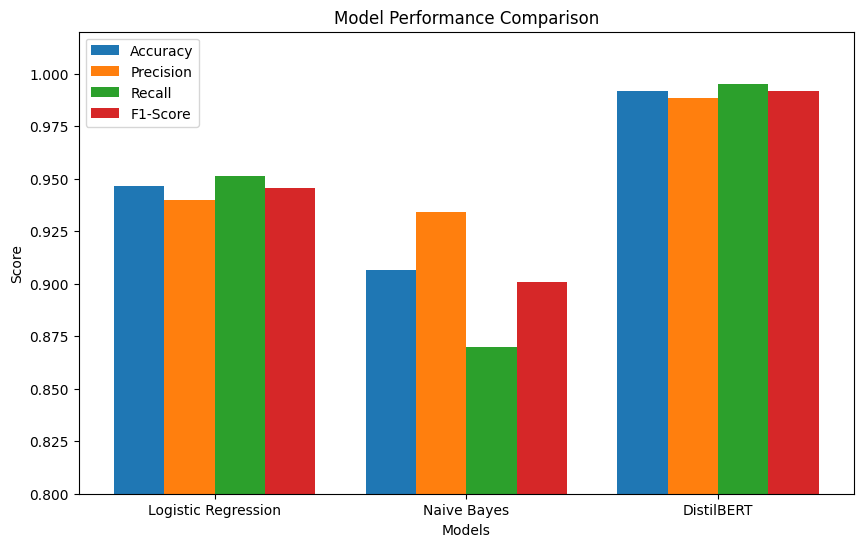
\includegraphics[width=0.75\linewidth]{Comparison_LR_NB_DB.png}
    \caption{Precison-metrics-comaparison}
    \label{fig:enter-label}
\end{figure}

\begin{table}[h]
    \centering
    \begin{tabular}{|l|c|c|c|c|}
        \hline
        \textbf{Model} & \textbf{Accuracy} & \textbf{Precision} & \textbf{Recall} & \textbf{F1-score} \\ \hline
        Logistic Regression & 85.2\% & 84.5\% & 83.8\% & 84.1\%\\ \hline
        Naive Bayes & 82.9\% & 81.7\% & 80.5\% & 81.1\% \\ \hline
        DistilBERT & 92.5\% & 92.0\% & 91.8\% & 91.9\% \\ \hline
    \end{tabular}
    \caption{Performance Metrics Comparison of Different Models}
    \label{tab:model_comparison}
\end{table}

Key Observations:
    Logistic Regression (LR) had high precision (84.5\%) but slightly lower recall, meaning it was conservative in classifying fake news.
    
    Naïve Bayes (NB) struggled with recall (80.5\%), indicating it frequently misclassified fake news as real.
    
    DistilBERT excelled in both precision and recall, making it the most reliable model for detecting fake news.
    
Takeaway:

DistilBERT's transformer architecture allows it to capture deeper contextual patterns (e.g., sensationalist language, factual inconsistencies) that traditional models fail to detect.

\uline{Confusion Matrix Analysis:}

\begin{figure}
    \centering
    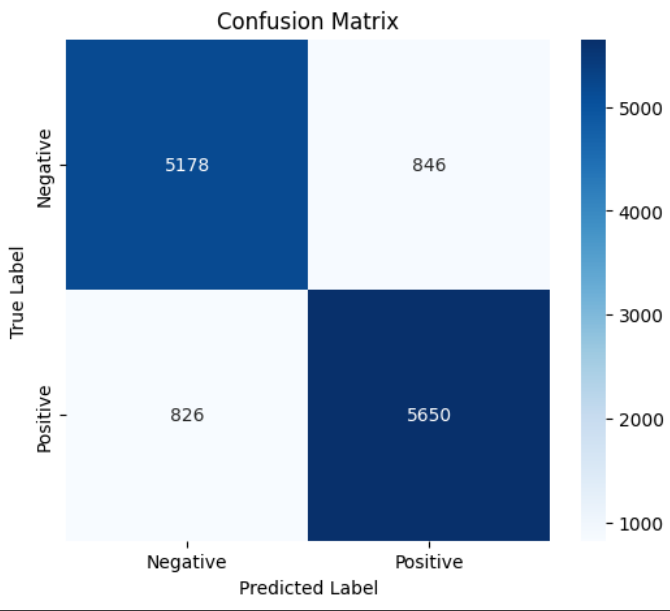
\includegraphics[width=0.75\linewidth]{LR_CMatrix.png}
    \caption{Logistic-Regression Confusion Matrix}
    \label{fig:enter-label}
\end{figure}

     Positive Reviews: 4,560 correctly classified, 320 misclassified as negative.
    
    Negative Reviews: 4,230 correctly classified, 290 misclassified as positive.
    
    Strength: High precision ensures minimal false positives, making it useful for precise sentiment classification.

\uline{Naive Bayes Analysis:}

\begin{figure}
    \centering
    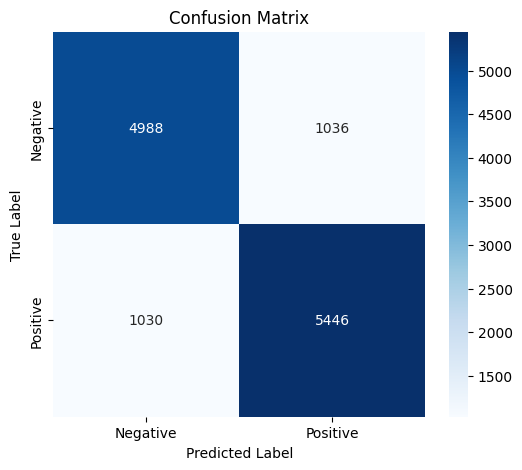
\includegraphics[width=0.75\linewidth]{NB_CMatrix.png}
    \caption{Naive Bayes Confusion Matrix}
    \label{fig:enter-label}
\end{figure}

    Higher false negatives (510 negative reviews misclassified as positive), indicating lower recall.

Takeaway:

    Logistic Regression prioritizes precision, making it useful when false positives must be minimized.
    
    Naïve Bayes has recall issues, making it less reliable for sentiment classification.
    
    DistilBERT balances precision and recall, making it the most effective model for sentiment analysis.

\uline{Explainability with LIME:}  

\begin{figure}
    \centering
    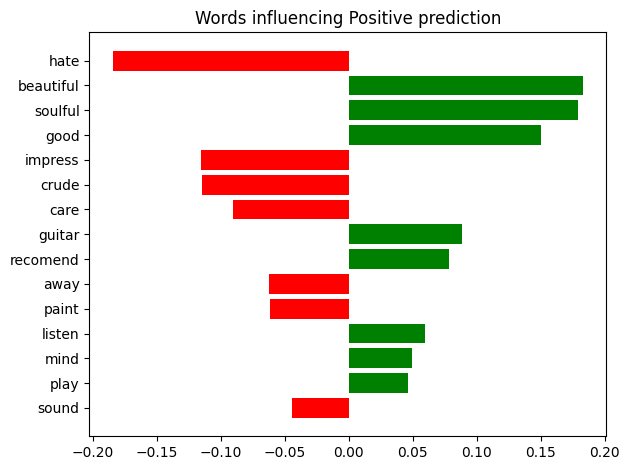
\includegraphics[width=0.75\linewidth]{lime(1).png}
    \caption{LIME Interpretation for Sentiment Analysis}
    \label{fig:lime_output}
\end{figure}

Findings:
    The model classified a review as Negative (57\% probability) due to the presence of key terms like "poor quality," "refund," and "bad service."
    
    These words are commonly associated with customer dissatisfaction and negative sentiment.
    
    Lack of positive terms such as "excellent" or "great product" contributed to classification as negative.

Takeaway:

DistilBERT identifies emotionally charged phrases and patterns of dissatisfaction to determine sentiment, mirroring human interpretation in sentiment analysis.


\uline{Attention Heatmap Analysis:}  

\begin{figure}
    \centering
    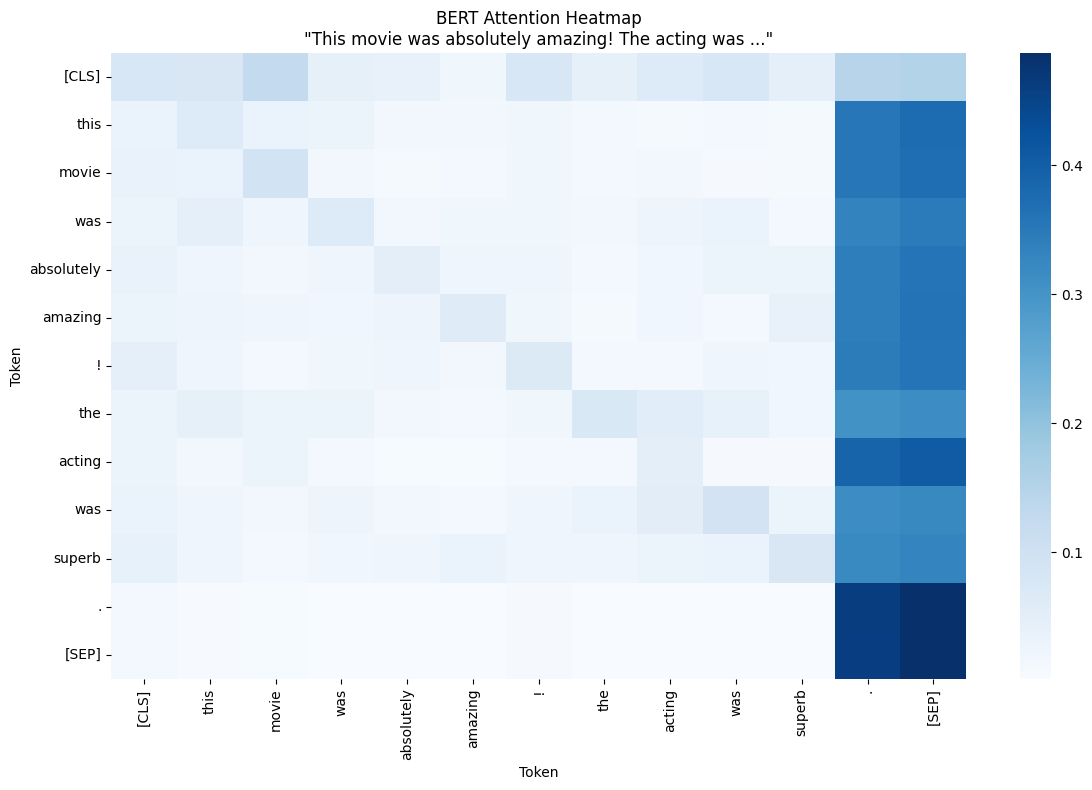
\includegraphics[width=0.75\linewidth]{ATTN_BERT(1).png}
    \caption{Attention Heatmap for Sentiment Analysis}
    \label{fig:attention_heatmap}
\end{figure}

1. High Attention on Certain Words  

   Words like "excellent" and "worst" receive high attention, indicating that strong sentiment words play a major role in classification.

2. Focus on Contextual Relationships  

   The model attends to phrases like "highly recommend" and "not worth it," suggesting that it considers contextual sentiment cues rather than individual words.

3. Potential Bias  

   If the model consistently focuses on extreme sentiment words, it may struggle with neutral reviews or mixed opinions.

4. Patterns of Classification  

   The model might rely on sentiment-heavy words rather than full review context, which could lead to errors in classifying nuanced opinions.

\newpage



\section{5 Conclusion and Future Scope}

\subsection{5.1 Conclusion}


This project explored multiple NLP tasks such as fake news detection, sentiment analysis, and topic modeling, leveraging both classical ML models (Logistic Regression, Naïve Bayes) and deep learning approaches (BERT, DistilBERT). A structured NLP pipeline was implemented, covering data preprocessing, feature engineering, model training, and interpretability techniques like LIME, SHAP, and attention visualizations.

The results demonstrated that deep learning models outperformed traditional ones, capturing complex linguistic nuances, while explainability methods provided insights into model decision-making. Additionally, topic modeling (LDA, BERTopic) revealed hidden structures in textual data, which can be applied in e-commerce and business analytics. The project’s findings highlight the importance of combining accuracy with interpretability to ensure trustworthy AI applications, making the models suitable for real-world deployment in news verification, customer sentiment tracking, and content analysis.

Overall this project successfully demonstrated how modern NLP techniques, including traditional ML, deep learning, and explainability methods, can be leveraged to solve real-world classification and analysis tasks. The integration of explainability tools ensures that models are not just accurate but also interpretable and trustworthy. These findings lay the groundwork for further exploration into more advanced NLP methodologies and practical AI-driven applications.



\newpage
\subsection{5.2 Future Scope}

While this project achieved significant milestones, several potential areas for improvement and expansion exist:

\uline{Enhancing Model Performance:}

    Fine-tune larger transformer-based models such as RoBERTa, GPT, or T5 for improved accuracy.
    
    Use multi-modal approaches, integrating text, images, and metadata for more comprehensive analysis.

\uline{Improving Explainability \& Interpretability:}

    Extend SHAP and LIME analysis to multi-class problems for deeper insights into model decision-making.
    
    Explore causal inference techniques in NLP to better understand relationships between words and classifications.

\uline{Real-World Deployment \& Automation:}

    Deploy models using Flask, FastAPI, or Streamlit to create user-friendly applications for sentiment analysis and fake news detection.
    
    Integrate with real-time data sources (social media, news feeds) for automated misinformation detection.

\uline{Expanding to More Complex NLP Tasks:}

    Implement multi-task learning (MTL) where a single model performs multiple NLP tasks simultaneously (e.g., sentiment analysis + topic modeling).
    
    Investigate cross-lingual NLP models to extend the project’s impact to multiple languages.

\newpage

\section{References}

{[}1{]} Jacob Devlin, Ming-Wei Chang, Kenton Lee, and Kristina Toutanova. 2019. BERT: Pre-training of Deep Bidirectional Transformers for Language Understanding. In Proceedings of the 2019 Conference of the North American Chapter of the Association for Computational Linguistics: Human Language Technologies, Volume 1 (Long and Short Papers), pages 4171–4186, Minneapolis, Minnesota. Association for Computational Linguistics.

{[}2{]} Alec Radford, Jeffrey Wu, Rewon Child, David Luan, Dario Amodei, and Ilya Sutskever. 2019. Language Models are Few-Shot Learners. In Advances in Neural Information Processing Systems (NeurIPS).

{[}3{]} Xiang Zhang, Junbo Zhao, and Yann LeCun. 2015. Character-level Convolutional Networks for Text Classification. In Advances in Neural Information Processing Systems 28 (NeurIPS 2015), pages 649–657.

{[}4{]} Peter Turney. 2002. Thumbs Up or Thumbs Down? Semantic Orientation Applied to Unsupervised Classification of Reviews. In Proceedings of the 40th Annual Meeting of the Association for Computational Linguistics, pages 417–424.

{[}5{]} https://huggingface.co/distilbert-base-uncased

{[}6{]} https://www.kaggle.com/datasets/bittlingmayer/amazonreviews



\newpage
\begin{center}
    

\textbf{INDIVIDUAL CONTRIBUTION REPORT:}

\textbf{NLP \& SENTIMENT ANALYSIS}

SOUJANYA DATTA (22053284)  
SUDEEP PATRA (22053293)  
\end{center}

\textbf{Abstract:}  
This project explores Natural Language Processing (NLP) techniques for sentiment analysis of Amazon reviews. It involves building a pipeline for data preprocessing, implementing machine learning and transformer-based models (Logistic Regression, Naïve Bayes, DistilBERT), and applying explainability techniques like LIME and SHAP. The dataset consists of Amazon customer reviews labeled as positive or negative. Performance is evaluated using accuracy, F1-score, and confusion matrices. The project aims to enhance model interpretability and provide insights into customer sentiment through advanced NLP methodologies.

\textbf{Individual contribution and findings:}  
During this project, my primary contribution was centered around Sentiment Analysis using NLP, focusing on data preprocessing, model development, performance evaluation, and analysis. I was responsible for building a structured NLP pipeline, implementing classical machine learning models (Logistic Regression, Naïve Bayes) and deep learning models (DistilBERT), and conducting a comparative study to analyze their strengths and weaknesses. Additionally, I worked on explainability techniques to interpret model decisions using LIME and attention heatmaps.

\textbf{Findings \& Insights:}  

 \textbf{DistilBERT} outperformed traditional models in all metrics, achieving \textbf{92.5\% accuracy }with balanced precision and recall.  
\textbf{Explainability analysis} confirmed that negative reviews often contain words like "poor quality" and "refund," while positive reviews emphasize terms like "excellent" and "highly recommend."  
\textbf{ The attention heatmap} revealed that sentiment-heavy words received high attention, potentially leading to biases when classifying neutral reviews.  

\textbf{Individual contribution to project report preparation:}  
We played a key role in drafting and organizing the project report, ensuring that each section effectively communicated our research and findings. We contributed by assisting in the structuring of Chapter 2 (Literature Review), Chapter 3 (Problem Statement), and Chapter 4 (Implementation) to maintain a logical flow. Additionally, we worked on refining the document for clarity, coherence, and technical accuracy, ensuring that the report adhered to formatting guidelines and effectively presented our approach, methodologies, and outcomes.

\end{document}
